\begin{definition}[Konform avbildning]

\end{definition}

\begin{example}
	Exempel på konform avbildning.
\end{example}




\begin{definition}[Konform ekvivalens]

\end{definition}


\begin{theorem}\label{thm:öppna_områden_bevaras}
	Öppna områden, samt enkelt sammanhängande områden bevaras under en holomorf avbildning.
\end{theorem}

\begin{theorem}[Maximumprincipen]
    \label{thm:maximumprincipen}
	Låt $\Omega$ vara ett öppet sammanhängande område. Antag att $f \in \H(\Omega)$ och kontinuerlig på $\overline{\Omega}$. Om $f$ inte är konstant så antar $\abs{f}$ max på $\partial \Omega$.
\end{theorem}
\begin{proof}
	Vi visar det kontrapositiva påståendet. Antag att $z_0 \in \Omega$ och att $\abs{f(z_0)}$ är ett lokalt maximum av $\abs{f}$. Eftersom $\Omega$ är öppen kan vi skapa en sluten cirkelskiva $D(z_0, R) \subset \Omega$, där det enligt antagandet gäller att
	\begin{equation}\label{eq:max_princ_assump}
		\abs{f(z)} \le \abs{f(z_0)} \quad \forall z \in D.
	\end{equation}
	I cirkelskivan gäller för varje $0 < r \le R$ enligt medelvärdesegenskap att
	\begin{equation*}
		f(z_0) = \frac{1}{2\pi} \int_0^{2\pi}{f(z_0 + re^{i\theta}) d\theta}.
	\end{equation*}
	Enligt triangelolikheten får vi att
	\begin{align*}
		\abs{f(z_0)} & \le \frac{1}{2\pi} \int_0^{2\pi}{\underbrace{\abs{f(z_0+ re^{i\theta})}}_{\le \abs{f(z_0)}} d\theta} \\
		             & \le \frac{1}{2\pi} \int_0^{2\pi}{\abs{f(z_0)} d\theta} = \abs{f(z_0)},
	\end{align*}
	där andra olikheten gäller enligt antagandet \eqref{eq:max_princ_assump}. Likheten i sista steget ger att
	\begin{align*}
		\int_0^{2\pi}{\abs{f(z_0)} d\theta}                                  & =  \int_0^{2\pi}{\abs{f(z_0 + re^{i\theta})} d\theta} \\
		\iff \int_0^{2\pi}{\abs{f(z_0)}-\abs{f(z_0 + re^{i\theta})} d\theta} & = 0.
	\end{align*}
	Eftersom integranden är större än 0 enligt antagandet, och det är en kontinuerlig funktion så måste
	\begin{align*}
		\abs{f(z_0)} - \abs{f(z_0 + re^{i\theta})} & = 0                                                                             \\
		\iff \abs{f(z_0)}                          & = \abs{f(z)} = \text{konstant} \overset{\text{def}}{=} M \quad \forall z \in D.
	\end{align*}
	% Det följer ur Identitessatsen för holomorfa funktioner att
	% \begin{equation*}
	% 	\abs{f(z)} = \abs{f(z_0)} = \text{konstant} \overset{\text{def}}{=} M \quad \forall z \in \mathbb{C}.
	% \end{equation*}
	Vi visar nu att även $f(z)$ måste vara konstant på $D$. Från ekvationen ovan kan vi skriva
	\begin{equation*}
		\abs{f(z)}^2 = f(z)\conj{f(z)} = M^2.
	\end{equation*}
	Fallet $M=0$ ger direkt $f(z) \equiv 0$. Om $M\neq 0 $ så är $f(z) \neq 0$ och likheten ovan kan skrivas
	\begin{equation*}
		\conj{f(z)} = \frac{M^2}{f(z)},
	\end{equation*}
	som blir en holomorf funktion, eftersom $f$ var holomorf. Både $f$ och $\conj{f}$ måste alltså uppfylla Cauchy-Riemanns ekvationer, och sätter man in
	\begin{equation*}
		f(z) = u(x, y) + iv(x, y) \quad \text{och} \quad \conj{f(z)} = u(x, y) - iv(x, y)
	\end{equation*}
	får man direkt att $u$ och $v$ är konstanta. Därför är $f(z)$ konstant på $D$ och eftersom cirkelskivan innehåller hopningspunkter följer av Identitetsatsen för holomorfa funktioner att $f(z)$ är konstant i $\Omega$.
\end{proof}

\begin{lemma}[Schwarz lemma]
    Antag att $f \in \H$. Om $\abs{f(z)} \le 1$ och $f(0)=0$ så gäller
    \begin{align*}
        \abs{f(z)} &\le \abs{z} \quad z \in U \text{, och} \\
        \abs{f'(0)} &\le 1.
    \end{align*}
\end{lemma}

\begin{proof}
    Bilda funktionen $f_r(z) = f(rz)$ för något $0 < r 1$. Vi ser sedan till funktionen $f_r(z)/z$, vilken (eftersom $f_r(0)=0$) har en hävbar singularitet i $z=0$. Vi får därför att $f_r(z)/z \in \H(U) \cap C(\overline{U}$). Vi uttnyttjar nu maximumprincipen \ref{thm:maximumprincipen} för att säga
    \begin{equation*}
        \abs{f_r(z)/z} \le \sup_{\abs{\zeta} = 1} \abs{f_r(\zeta)/\zeta} \le 1, \quad z \in U.
    \end{equation*}
    Genom multiplikation av $\abs{z}$ erhålles $\abs{f_r(z)} \le \abs{z}$. Låter vi $r$ gå mot 1 ser vi att $\abs{f(z)} \le \abs{z}$. Vi bildar nu funktionen $g(z) := f(z)/z$ och utvärderar denna i den hävbara singulariteten $z=0$ för att få
    \begin{equation*}
        g(0) = \lim_{z \to 0} \frac{f(z) - f(0)}{z - 0} = f'(0).
    \end{equation*}
    Från att $\abs{g(z)} \le 1$ (speciellt för $z=0$) följer att $f'(0) \le 1$.
\end{proof}

\begin{lemma}
    Funktionen $\phi_\alpha = \dfrac{z - \alpha}{1 - \conj{\alpha}z}$, där $\abs{\alpha} < 1$, avbildar den öppna enhetsdisken på sig själv.
\end{lemma}

\begin{proof}
    Vi börjar med att visa att $\phi_\alpha$ avbildar randen till enhetsdisken på sig själv. Då $z = e^{i \theta}$ ser vi att
    \begin{equation*}
        \abs{\phi_\alpha(e^{i \theta})} = \abs{\frac{e^{i \theta} - \alpha}{1 - \conj{\alpha}e^{i \theta}}} = \frac{\abs{e^{i \theta}}\abs{1 - \alpha e^{-i \theta}}}{\abs{1- \conj{\alpha}e^{i\theta}}}
    \end{equation*}
    Genom att ta konjugatet av täljaren får vi
    \begin{equation*}
        \abs{\phi_\alpha(e^{i \theta})} = \frac{\abs{1 - \conj{\alpha} e^{i \theta}}}{\abs{1- \conj{\alpha}e^{i\theta}}} = 1
    \end{equation*}
    Randen avbildas på sig själv. Vi får från maximumprincipen \ref{thm:maximumprincipen} att maximum för $\abs{\phi_\alpha}$ på $U$ kommer att antas på randen till $U$. Alltså
    \begin{equation*}
        \abs{\phi_\alpha(z)} \le 1 \quad z \in U.
    \end{equation*}
    Lemmat följer från detta tillsammans med att funktionen bevarar att enhetsdisken är öppen, enkel och sammanhängande.
\end{proof}

\begin{proof}
    Tag punkt på randen. Betrakta absolutbelopp och bryt ut punkten. Konjugera täljaren. Se att absoluten är 1. Det har hamnat på randen. Absolutbelopp av en holomorf funktion antar sitt max på randen. Alltså måste inre punkter ha hamnet i det inre till enhetsdisken. 
\end{proof}

\begin{theorem}[Riemanns avbildningssats]
	Varje enkelt sammanhängande område $\Omega \subset \mathbb{C}$ är konformt ekvivalent med den öppna enhetsdisken $U$.
\end{theorem}

\begin{proof}
	Låt $\Omega \subset \mathbb{C}$ vara ett enkelt sammanhängande område och $w_0$ en punkt utanför $\Omega$. Bilda mängden
	\begin{equation*}
		\Sigma = \{ \Psi \in \H(\Omega) \mid \Psi \text{ injektiv på } \Omega \text{ och } \Psi \text{ lägger } \Omega \text{ i } U\}.
	\end{equation*}
	Med att $\Psi$ lägger $\Omega$ i $U$ menas att $\Psi(z) \in U$ för alla $z \in \Omega$.

	Vi börjar med att visa att mängden $\Sigma$ inte är tom -- det vill säga att det existerar någon funktion $\Psi$ som uppfyller dessa krav. Betrakta en funktion $\phi$ som uppfyller
	\begin{equation} \label{eq:phi^2}
		\phi^2(z) = z - w_0 \quad z \in \Omega.
	\end{equation}
	Att en sådan funktion faktiskt existerar följer av att $w_0$ inte ligger i $\Omega$, och att $\Omega$ är enkelt sammanhängande. Eftersom $w_0 \notin \Omega$ så är $z-w_0 \neq 0$. Alltså hamnar ingen punkt $z$ i origo efter translationen. Dessutom kommer inte det translaterade området att omsluta origo, eftersom $\Omega$ är enkelt sammanhängande. Detta innebär att det existerar någon gren av logaritm så att
	\begin{equation*}
		\phi(z) = (z-w_0)^{\frac{1}{2}} = e^{\frac{1}{2} \Log(z-w_0)}.
	\end{equation*}
	Beroende på hur $\Omega$ ser ut, kan vi behöva välja ett grensnitt som inte är en linje utan en kurva, se figur~\ref{fig:grensnitt_kurva}. Då kommer intervallet för argument som tillåts att ändras beroende på $\vert z \vert$, men fortfarande vara entydigt. Det finns alltså en funktion $\phi \in \H(\Omega)$ som uppfyller \eqref{eq:phi^2}.


	\begin{figure}
		\begin{center}
			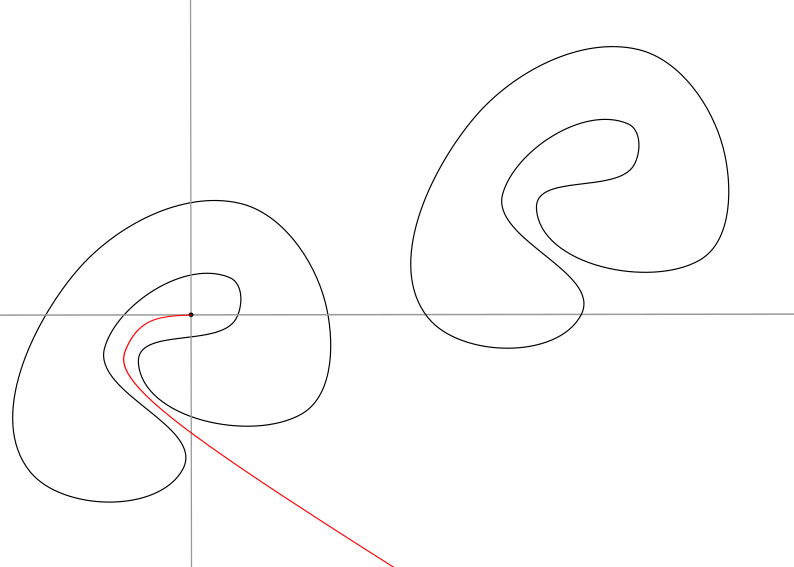
\includegraphics[width=0.95\textwidth]{figures/grensnitt.png}
		\end{center}
		\caption{Området $\Omega$ och $\Omega-w_0$. Det går att välja en kurva $\gamma$ som grensnitt. }\label{fig:grensnitt_kurva}
	\end{figure}


	Låt oss nu visa att $\phi$ också är injektiv. Tag $z_1, z_2 \in \Omega$. Då är enligt \eqref{eq:phi^2}
	\begin{equation*}
		\phi(z_1)^2 = z_1 - w_0 \quad \text{och} \quad \phi(z_2) = z_2 - w_0.
	\end{equation*}
	Sätter vi $\phi(z_1) = \phi(z_2)$ får vi att $z_1 = z_2$, vilket visar att $\phi$ är injektiv.

	På liknande sätt visar vi att
	\begin{equation}\label{eq:phi_symmetry}
		\nexists \quad z_1, z_2 \in \Omega \text{ så att } \phi(z_1) = -\phi(z_2).
	\end{equation}
	Antar vi likheten och kvadrerar båda sidor får vi enligt \eqref{eq:phi^2}
	\begin{equation*}
		z_1 - w_0 = z_2 - w_0 \iff z_1 = z_2.
	\end{equation*}
	Då måste $\phi(z_1) = -\phi(z_1)$ vilket endast kan vara uppfyllt då $\phi(z_1) = 0$. Då är även
	\begin{equation*}
		\phi(z_1)^2 = z_1 - w_0 = 0,
	\end{equation*}
	vilket endast är uppfyllt om $z_1 = w_0$. Detta motsäger att $z_1 \in \Omega$. Notera alltså att $0 \notin \phi(\Omega)$.



	Eftersom $\phi$ är holomorf är det enligt sats \ref{thm:öppna_områden_bevaras} en avbildning som bevarar öppna områden. Det innebär att det går att hitta en cirkelskiva $D(a, r) \in \phi(\Omega)$, med  $0< r < \vert a\vert$, se figur \ref{fig:phi(omega)-disk}. Denna begränsning på $r$ är inte någon inskränkning eftersom om vi skulle ha en cirkel med större radie än $\vert a\vert$ så gäller det även att en mindre cirkel också ligger i $\phi(\Omega)$. Vi kan även konstatera att cirkelskivan $D(-a, r)$ \emph{inte} ligger i $\phi(\Omega)$, till följd av \eqref{eq:phi_symmetry}. Bilda nu funktionen
	\begin{equation}
		\Psi(z) = \frac{r}{\phi(z) +a}.
	\end{equation}
	Det gäller att $\Psi \in \H(\Omega)$ och att $\Psi$ är injektiv. Vidare är
	\begin{equation*}
		\abs{\Psi(z)} = \abs{\frac{r}{\phi(z) +a}} =\frac{r}{\abs{\phi(z) - (-a)}} < 1,
	\end{equation*}
	ty $\abs{\phi(z) - (-a)} > r$ eftersom $D(-a, r) \notin \phi(\Omega)$. Alltså gäller det att $\Psi \in \Sigma$ och mängden är icketom.


	\begin{figure}
		\begin{center}
			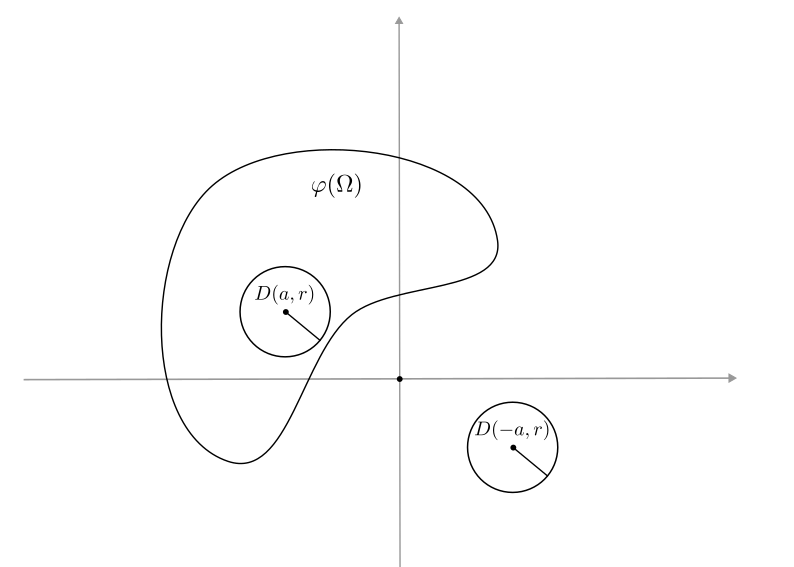
\includegraphics[width=0.95\textwidth]{figures/disk.png}
		\end{center}
		\caption{Eftersom $\phi(\Omega)$ är öppen finns en disk $D(a, r) \in \phi(\Omega)$. Disken $D(-a, r)$ ligger \emph{inte} i $\phi(\Omega)$.}\label{fig:phi(omega)-disk}
	\end{figure}


	Vi ska nu visa att om $\Psi \in \Sigma$ och $\Psi(\Omega)$ inte täcker hela $U$, och om $z_0 \in \Omega$ så går det att hitta en funktion $\tilde{\Psi}$ som uppfyller
	\begin{equation} \label{eq:psi_deriv_bigger}
		\abs{\tilde{\Psi}'(z_0)} > \abs{\Psi'(z_0)}.
	\end{equation}
	Vi inför en hjälpfunktion
	\begin{equation*}
		\phi_{\alpha}(z) = \frac{z-\alpha}{1-\conj{\alpha}z}, \quad \alpha \in \mathbb{C}.
	\end{equation*}
	Lite algebra visar att $\phi_{-\alpha}$ är dess invers:
	\begin{equation*}
		\phi_{\alpha} \circ \phi_{-\alpha} (z) = \phi_{\alpha} \left(\frac{z+\alpha}{1+\conj{\alpha}z}\right) = \frac{\frac{z+\alpha}{1+\conj{\alpha}z} - \alpha}{1 - \conj{a}\frac{z+\alpha}{1+\conj{\alpha}z}} = \frac{z+\alpha - \alpha - \alpha\conj{\alpha}z}{1+\conj{\alpha}z - \conj{\alpha}z - \alpha\conj{\alpha}} = \frac{z(1-\alpha\conj{\alpha})}{1 - \alpha\conj{\alpha}} = z.
	\end{equation*}
	Det gäller också att $\phi_{\alpha}$ är bijektiv mellan $U$ och $U$.

	Tag nu ett $\Psi \in \Sigma$, $\alpha \in U$ där $\alpha \notin \Psi(\Omega)$, se figur \ref{fig:psi_omega}. Då gäller att sammansättningen $\phi_{\alpha} \circ \Psi \in \Sigma$ eftersom funktionen är holomorf och injektiv på $\Omega$ samt att $\Psi$ mappar $\Omega$ inuti $U$ och $\phi_{\alpha}$ mappar $U$ på $U$.


	\begin{figure}
		\begin{center}
			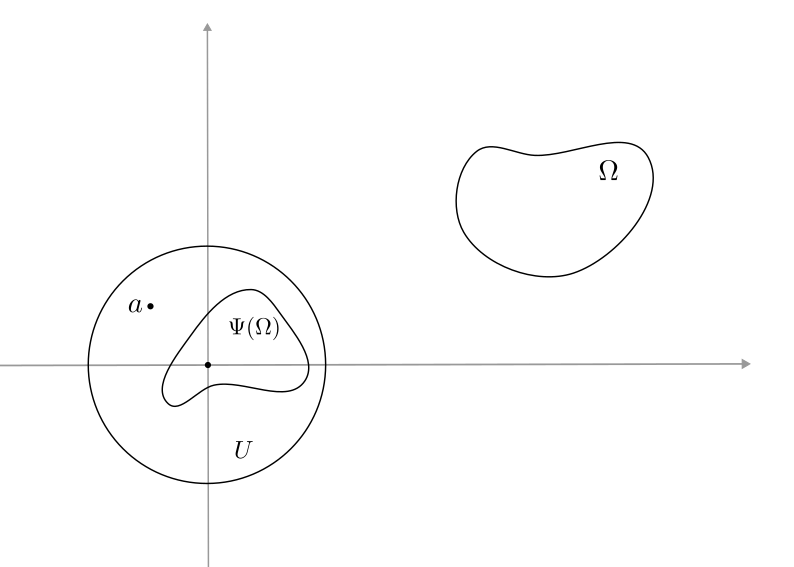
\includegraphics[width=0.95\textwidth]{figures/psi_omega.png}
		\end{center}
		\caption{}\label{fig:psi_omega}
	\end{figure}


	Eftersom $\alpha \notin \Psi(\Omega)$ har $\phi_{\alpha} \circ \Psi$ inget nollställe i $\Omega$ ty
	\begin{equation*}
		\phi_{\alpha}(z) = 0 \iff z = \alpha.
	\end{equation*}
	Det existerar därmed en funktion $g \in \H(\Omega)$ så att
	\begin{equation} \label{eq:g^2}
		g^2(z) = \phi_{\alpha} \circ \Psi(z),
	\end{equation}
	eftersom $g^2(\Omega)$ är enkelt sammanhängande och med samma argument som tidigare för att det går att definiera en logaritm. Dessutom är $g$ injektiv vilket ger oss att $g \in \Sigma$. Om vi definierar
	\begin{equation} \label{eq:psi-tilde}
		\Psi_1 = \phi_{\beta} \circ g,
	\end{equation}
	för något $\beta$, så kommer $\Psi_1 \in \Sigma$. Låter vi funktionen $s$ vara kvadratfunktionen, det vill säga $s(w) = w^2$ så kommer det enligt \eqref{eq:g^2} och \eqref{eq:psi-tilde} gälla att
	\begin{equation}\label{eq:relation_psi_psi-tilde}
		\Psi = \phi_{-\alpha} \circ s\circ g =\phi_{-\alpha} \circ s \circ \phi_{-\beta} \circ \Psi_1 = F \circ \Psi_1,
	\end{equation}
	där $F =\phi_{-\alpha} \circ s \circ \phi_{-\beta}$.
	Om vi väljer $\beta = g(z_0)$ är
	\begin{equation*}
		\Psi_1(z_0) = \phi_{\beta} \circ g(z_0) = \frac{g(z_0) - g(z_0)}{1- \conj{g(z_0)}z_0} = 0.
	\end{equation*}
	Därför får vi från \eqref{eq:relation_psi_psi-tilde} och kedjeregeln att
	\begin{equation*}
		\Psi'(z_0) = \Psi_1'(z_0)F'(\Psi_1(z_0))  = \Psi_1'(z_0)F'(0).
	\end{equation*}
	Vi ser att $F$ uppfyller kraven för Schwarz lemma vilket ger att $\abs{F'(0)} < 1$ och \eqref{eq:psi_deriv_bigger} är därmed uppfyllt.

	Vi ser att det för varje funktion i $\Sigma$ vars bild av $\Omega$ inte är hela $U$ existerar en funktion med större derivata i någon punkt $z_0$. Det kontraspositiva påståendet till detta ger oss att om vi finner en funktion som har den största derivatan i punkten $z_0$ så kommer denna funktionens bild av $\Omega$ att vara hela $U$. Vi definierar
	\begin{equation*}
		\eta = \sup \{ |\Psi'(z_0)| : \Psi \in \Sigma \}.
	\end{equation*}
	Eftersom $\Sigma$ inte är tom, och funktionerna däri är injektiva, följer att $\eta > 0$. Vi vet att $\Sigma$ är likformigt begränsad då $\abs{\Psi(z)} < 1$ då $z \in \Omega$. Därutöver ser vi att $\abs{\Psi'}$ är kontinuerlig på kompakta delmängder till $\Omega$, varav det följer från Weierstra\ss~extremvärdessats att $\abs{\Psi'}$ är begränsad. Därmed existerar $\eta$ enligt supremumaxiomet.

	Det existerar enligt supremumaxiomet en följd $\{\abs{\Psi'_n(z_0)}\}$ som konvergerar till $\eta$. Eftersom $\Sigma$ är likformigt begränsad följder det att det är en normalfamilj. Ur följden $\Psi_n$ kan vi därför ta en delföljd $\Psi_k$ så att $\Psi_k \xrightarrow{u} \zeta$ för någon funktion $\zeta$.

	Det följer av att $\Psi_k \xrightarrow{u} \zeta$ och att $\Psi_k$ är holomorfa att $\Psi'_k \xrightarrow{u} \zeta'$. Följden $\{\abs{\Psi'_k(z_0)}\}$, vilken konvergerar till $\abs{\zeta'(z_0)}$, är därför en delföljd till $\{\abs{\Psi'_n(z_0)}\}$ vilken konvergerar till $\eta$. Det följer att $\abs{\zeta'(z_0)}=\eta$.

	Låt oss nu visa att $\zeta$ ligger i $\Sigma$ och att den därmed lägger $\Omega$ på $U$. Eftersom $\zeta$ har nollskild derivata i $z_0$ följer det att den inte är konstant. Vi kan då med sats (sats som ska skrivas i framtiden) säga att $\zeta$ är injektiv. Det återstår nu endast att se att den lägger $\Omega$ på $U$. Per definition gäller det att $\Psi_k(\Omega) \subset U$. Antag att det för något $z$ skulle gälla att $\zeta(z) \notin \overline{U}$. Vi kan då inte finna något $z'$ så att
	\begin{equation*}
		\abs{\Psi(z') - \zeta(z)} < \epsilon
	\end{equation*}
	då $n \to \infty$ för godtyckligt litet $\epsilon$. Alltså måste $\zeta(\Omega) \subset \overline{U}$. Men då $\zeta$ är holomorf och $\Omega$ öppen gäller enligt sats \ref{thm:öppna_områden_bevaras} att $\zeta(\Omega) \subset U$. Det följer att $\zeta \in \Sigma$ och eftersom $\zeta'(z_0) = \eta$ lägger $\zeta$ området $\Omega$ på $U$.
\end{proof}

\section{Frågor till Mikael Persson Sundqvist}
\begin{itemize}
	\item Vilken form av Schwarz lemma är det som ska användas? Funktionen $F$ uppfyller icke att $F(0)=0$.
	\item Krävs injektivitet för att holomorfa funktioner ska bevara öppna, sammanhängande områden.
\end{itemize}
